

% This is "sig-alternate.tex" V1.9 April 2009
% This file should be compiled with V2.4 of "sig-alternate.cls" April 2009
%
% This example file demonstrates the use of the 'sig-alternate.cls'
% V2.4 LaTeX2e document class file. It is for those submitting
% articles to ACM Conference Proceedings WHO DO NOT WISH TO
% STRICTLY ADHERE TO THE SIGS (PUBS-BOARD-ENDORSED) STYLE.
% The 'sig-alternate.cls' file will produce a similar-looking,
% albeit, 'tighter' paper resulting in, invariably, fewer pages.
%
% ----------------------------------------------------------------------------------------------------------------
% This .tex file (and associated .cls V2.4) produces:
%       1) The Permission Statement
%       2) The Conference (location) Info information
%       3) The Copyright Line with ACM data
%       4) NO page numbers
%
% as against the acm_proc_article-sp.cls file which
% DOES NOT produce 1) thru' 3) above.
%
% Using 'sig-alternate.cls' you have control, however, from within
% the source .tex file, over both the CopyrightYear
% (defaulted to 200X) and the ACM Copyright Data
% (defaulted to X-XXXXX-XX-X/XX/XX).
% e.g.
% \CopyrightYear{2007} will cause 2007 to appear in the copyright line.
% \crdata{0-12345-67-8/90/12} will cause 0-12345-67-8/90/12 to appear in the copyright line.
%
% ---------------------------------------------------------------------------------------------------------------
% This .tex source is an example which *does* use
% the .bib file (from which the .bbl file % is produced).
% REMEMBER HOWEVER: After having produced the .bbl file,
% and prior to final submission, you *NEED* to 'insert'
% your .bbl file into your source .tex file so as to provide
% ONE 'self-contained' source file.
%
% ================= IF YOU HAVE QUESTIONS =======================
% Questions regarding the SIGS styles, SIGS policies and
% procedures, Conferences etc. should be sent to
% Adrienne Griscti (griscti@acm.org)
%
% Technical questions _only_ to
% Gerald Murray (murray@hq.acm.org)
% ===============================================================
%
% For tracking purposes - this is V1.9 - April 2009

\documentclass{sig-alternate}
  \pdfpagewidth=8.5truein
  \pdfpageheight=11truein

\usepackage[latin1]{inputenc}
\usepackage{graphicx}
\usepackage{color}
\usepackage{url}
\usepackage[english]{babel}

\begin{document}
%
% --- Author Metadata here ---
\conferenceinfo{SAC'14}{March 24-28, 2014, Gyeongju, Korea.}
\CopyrightYear{2014} % Allows default copyright year (2002) to be over-ridden - IF NEED BE.
\crdata{978-1-4503-2469-4/14/03}  % Allows default copyright data (X-XXXXX-XX-X/XX/XX) to be over-ridden.
% --- End of Author Metadata ---

\title{MUSES: A corporate user-centric system which applies computational intelligence methods}
\subtitle{[Poster paper]}
%
% You need the command \numberofauthors to handle the 'placement
% and alignment' of the authors beneath the title.
%
% For aesthetic reasons, we recommend 'three authors at a time'
% i.e. three 'name/affiliation blocks' be placed beneath the title.
%
% NOTE: You are NOT restricted in how many 'rows' of
% "name/affiliations" may appear. We just ask that you restrict
% the number of 'columns' to three.
%
% Because of the available 'opening page real-estate'
% we ask you to refrain from putting more than six authors
% (two rows with three columns) beneath the article title.
% More than six makes the first-page appear very cluttered indeed.
%
% Use the \alignauthor commands to handle the names
% and affiliations for an 'aesthetic maximum' of six authors.
% Add names, affiliations, addresses for
% the seventh etc. author(s) as the argument for the
% \additionalauthors command.
% These 'additional authors' will be output/set for you
% without further effort on your part as the last section in
% the body of your article BEFORE References or any Appendices.


%>>>\numberofauthors{8} %  in this sample file, there are a *total*
% of EIGHT authors. SIX appear on the 'first-page' (for formatting
% reasons) and the remaining two appear in the \additionalauthors section.
%
%>>>\author{
% You can go ahead and credit any number of authors here,
% e.g. one 'row of three' or two rows (consisting of one row of three
% and a second row of one, two or three).
%
% The command \alignauthor (no curly braces needed) should
% precede each author name, affiliation/snail-mail address and
% e-mail address. Additionally, tag each line of
% affiliation/address with \affaddr, and tag the
% e-mail address with \email.
%
% 1st. author
%>>>\alignauthor
%Ben Trovato\titlenote{Dr.~Trovato insisted his name be first.}\\
%       \affaddr{Institute for Clarity in Documentation}\\
%       \affaddr{1932 Wallamaloo Lane}\\
%       \affaddr{Wallamaloo, New Zealand}\\
%       \email{trovato@corporation.com}
% 2nd. author
%\alignauthor G.K.M. Tobin\titlenote{The secretary disavows
%any knowledge of this author's actions.}\\
%       \affaddr{Institute for Clarity in Documentation}\\
%       \affaddr{P.O. Box 1212}\\
%       \affaddr{Dublin, Ohio 43017-6221}\\
%       \email{webmaster@marysville-ohio.com}
% 3rd. author
%\alignauthor Lars Th{\o}rv{\"a}ld\titlenote{This author is the
%one who did all the really hard work.}\\
%       \affaddr{The Th{\o}rv{\"a}ld Group}\\
%       \affaddr{1 Th{\o}rv{\"a}ld Circle}\\
%       \affaddr{Hekla, Iceland}\\
%       \email{larst@affiliation.org}
%\and  % use '\and' if you need 'another row' of author names
% 4th. author
%\alignauthor Lawrence P. Leipuner\\
%       \affaddr{Brookhaven Laboratories}\\
%       \affaddr{Brookhaven National Lab}\\
%       \affaddr{P.O. Box 5000}\\
%       \email{lleipuner@researchlabs.org}
% 5th. author
%\alignauthor Sean Fogarty\\
%       \affaddr{NASA Ames Research Center}\\
%       \affaddr{Moffett Field}\\
%       \affaddr{California 94035}\\
%       \email{fogartys@amesres.org}
% 6th. author
%\alignauthor Charles Palmer\\
%       \affaddr{Palmer Research Laboratories}\\
%       \affaddr{8600 Datapoint Drive}\\
%       \affaddr{San Antonio, Texas 78229}\\
%       \email{cpalmer@prl.com}
%}
% There's nothing stopping you putting the seventh, eighth, etc.
% author on the opening page (as the 'third row') but we ask,
% for aesthetic reasons that you place these 'additional authors'
% in the \additional authors block, viz.
%>>>\additionalauthors{Additional authors: John Smith (The
%Th{\o}rv{\"a}ld Group, email: {\texttt{jsmith@affiliation.org}})
%and Julius P.~Kumquat (The Kumquat Consortium, email:
%{\texttt{jpkumquat@consortium.net}}).}
%\date{30 July 1999}
% Just remember to make sure that the TOTAL number of authors
% is the number that will appear on the first page PLUS the
% number that will appear in the \additionalauthors section.


\maketitle
\begin{abstract}
This work presents the description of a novel enterprise security system, still in development, which can deal with the recent situation inside the companies, the Bring Your Own Device (BYOD) philosophy. Thus, the Multiplatform Usable Endpoint Security system (MUSES) considers diverse factors such as the information distribution, the type of accesses, the context where the users are, the category of users, or the mix between personal and private data, among others.
This system includes a risk and trust analysis engine to aid in the decision process. MUSES follows a set of defined security rules, according to the enterprise security policies, but it is able to self-adapt the decisions and even create new security rules depending on the user behaviour, the specific device, and the situation or context. To this aim MUSES applies machine learning and computational intelligence techniques which can also be used to perform predictions on potential unsafe or dangerous user's behaviour.
\end{abstract}

%A category including the fourth, optional field follows...
\category{C.0}{Computer Systems Organization}{GENERAL}
% A category with the (minimum) three required fields
\category{K.6.5}{Computing Milieux}{MANAGEMENT OF COMPUTING AND INFORMATION SYSTEMS}[Security and Protection]

\terms{Security}

\keywords{enterprise security, BYOD, multiplatform, user-centric system, self-adaptation}

%
%%%%%%%%%%%%%%%%%%%%%%%%%%%%%%%   INTRODUCTION   %%%%%%%%%%%%%%%%%%%%%%%%%%%%%%%
%
\section{Introduction}
\label{sec:intro}

Some years ago, company data were stored in own servers which were accessed by the employees or users by means of desktop or portable computers. Nowadays it is frequent that these data are distributed among multiple machines, even not all belonging to the company, and being consulted and modified through a wide amount of devices, some of them owned by the company's users. This is the so-called Bring Your Own Device (BYOD) philosophy. It is becoming highly successful due to the impact that smartphones and tablets are having in the market.
Data security and privacy are key factors for a company, thus, to protect them, it is usual to define Organisational Security Policies. Their definition is nowadays a very difficult problem, since the BYOD tendency means that several factors must be considered \cite{Opp_Security11}, most of them previously ignored or non-considered in the security systems, for instance the current mixture between personal and professional information in these devices (the user could navigate inside social networks where there could be friends and also company partners or clients).

Moreover, it has been demonstrated that people are the main hazard regarding the company security \cite{Adams_Users05}, so in this situation, some monitorization and security-aimed applications are arising. Most of them try to be non-intrusive (regarding the users' personal data), friendly and easy to manage.
This work presents one of these systems, named MUSES, Multiplatform Usable Endpoint Security system. It is being implemented inside an European project and will provide a device independent, user-centric, and self-adaptive corporate security system, able to cope with the concept of seamless working experience on different devices. This concept is a methodology of work which allows users to start/continue a working session over multiple devices and locations without any significant loss of data. This new situation has a big impact from the point of view of the security \cite{Schu_SecPatterns05}, since the company's data borders have changed in the last years so now the users can access significant data from outside the enterprise, and possibly through a non absolutely secure channel.

In this scenario MUSES will analyse the users' behaviour and predict, using computational intelligence methods, risky or dangerous actions regarding both an event correlation and a risk and trust analysis engines. The system will be able to learn from the past user's behaviour, and react in a non-intrusive way to the potentially dangerous sequence of actions that he or she is conducting at any time.


%
%%%%%%%%%%%%%%%%%%%%%%%%%%%%   SYSTEM DESCRIPTION   %%%%%%%%%%%%%%%%%%%%%%%%%%%%
%
\section{System description}
\label{sec:system}

MUSES system will work as presented in Figure \ref{fig:system_overview}. The user interacts with the devices, own or corporate, through the MUSES graphical interface and inside his or her own context (situation, connection, status). This application includes two modules, a \textit{controller} and an \textit{actuator}. The first one monitorizes the environment (context) and the user's behaviour, translating his/her actions into a sequence of events. These events, along with the patterns defining the user's conduct, are processed by the system in real-time by means of a Risk and Trust Analysis Engine (RT2AE) and an Event Correlation module. Then, a decision is taken in the corporate security operations centre (SOC) side, considering the RT2AE output and the set of security rules adapted to that specific user and context. The correspondent feedback is communicated to the user through the \textit{actuator}, which is also in charge of triggering the recommended actions to stop the user's or application's doings, in case it is required.

\begin{figure}
\centering
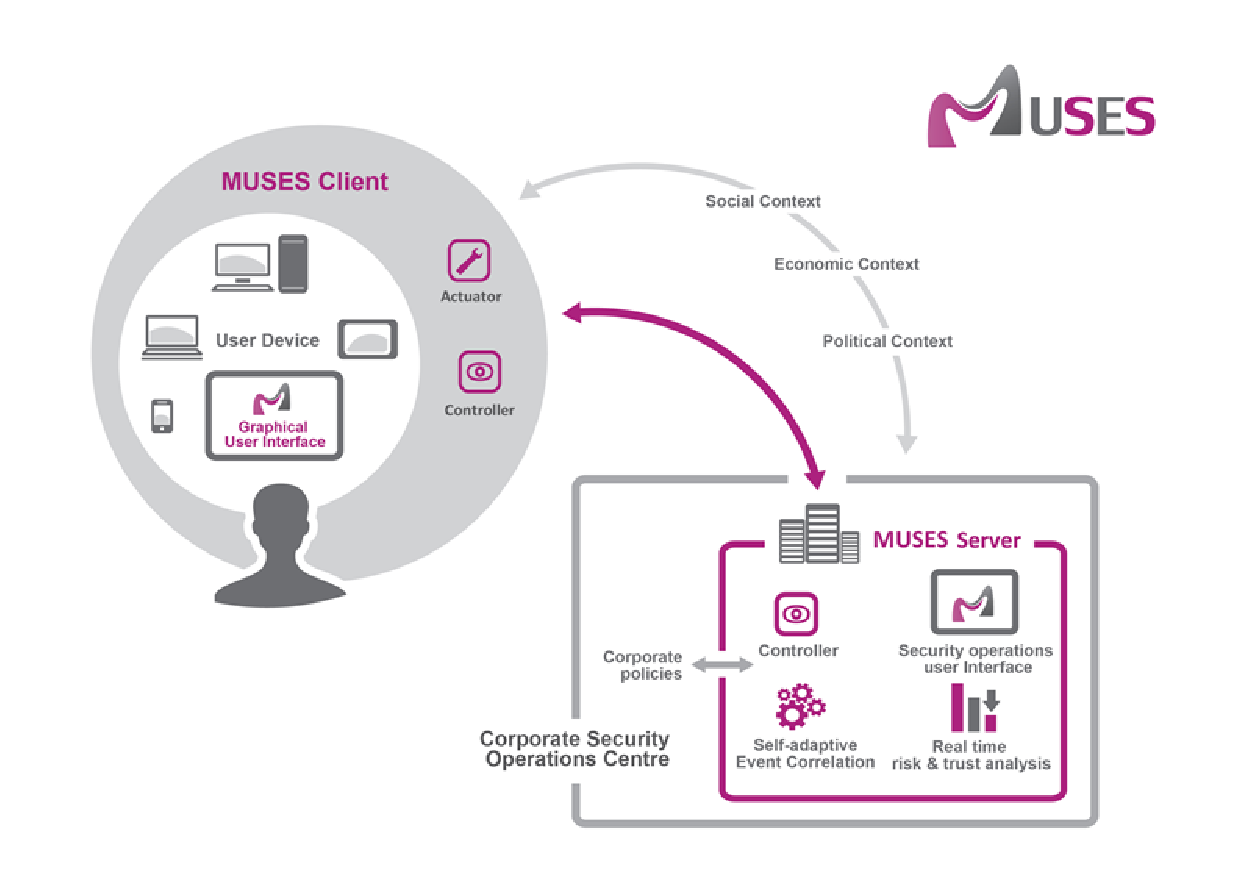
\epsfig{file=system_overview.eps, scale=0.45}
\caption{MUSES system overview.\label{fig:system_overview}}
\end{figure}

The system architecture can be seen in Figure \ref{fig:architecture}. It is a client-server approach in which the \textit{client} program will be installed in every user's device independently of the platform (operative system and type of device). This client contains a \textit{monitorization module}, which gathers the performed sequence of events and user context information; a \textit{controller module} in charge of take some light decisions considering the server response to the current situation (it will also take the control in case the device cannot connect with the server). The device controller will trigger the \textit{actuator} if necessary. This module will provide the user with some feedback, and will interact with the applications being monitorized if recommended or required.

The \textit{server} side would be installed in the corporate SOC. This application contains, in addition to an user interface to manage it, the main modules in the security-aimed decision process: the \textit{RT2AE} and the \textit{Event Correlator}. These components are connected between them and also with the main \textit{Controller}, that will connect with the device side sending the selected set of security rules that better fit with the current situation, along with the actions to be performed according to them.

\begin{figure}
\centering
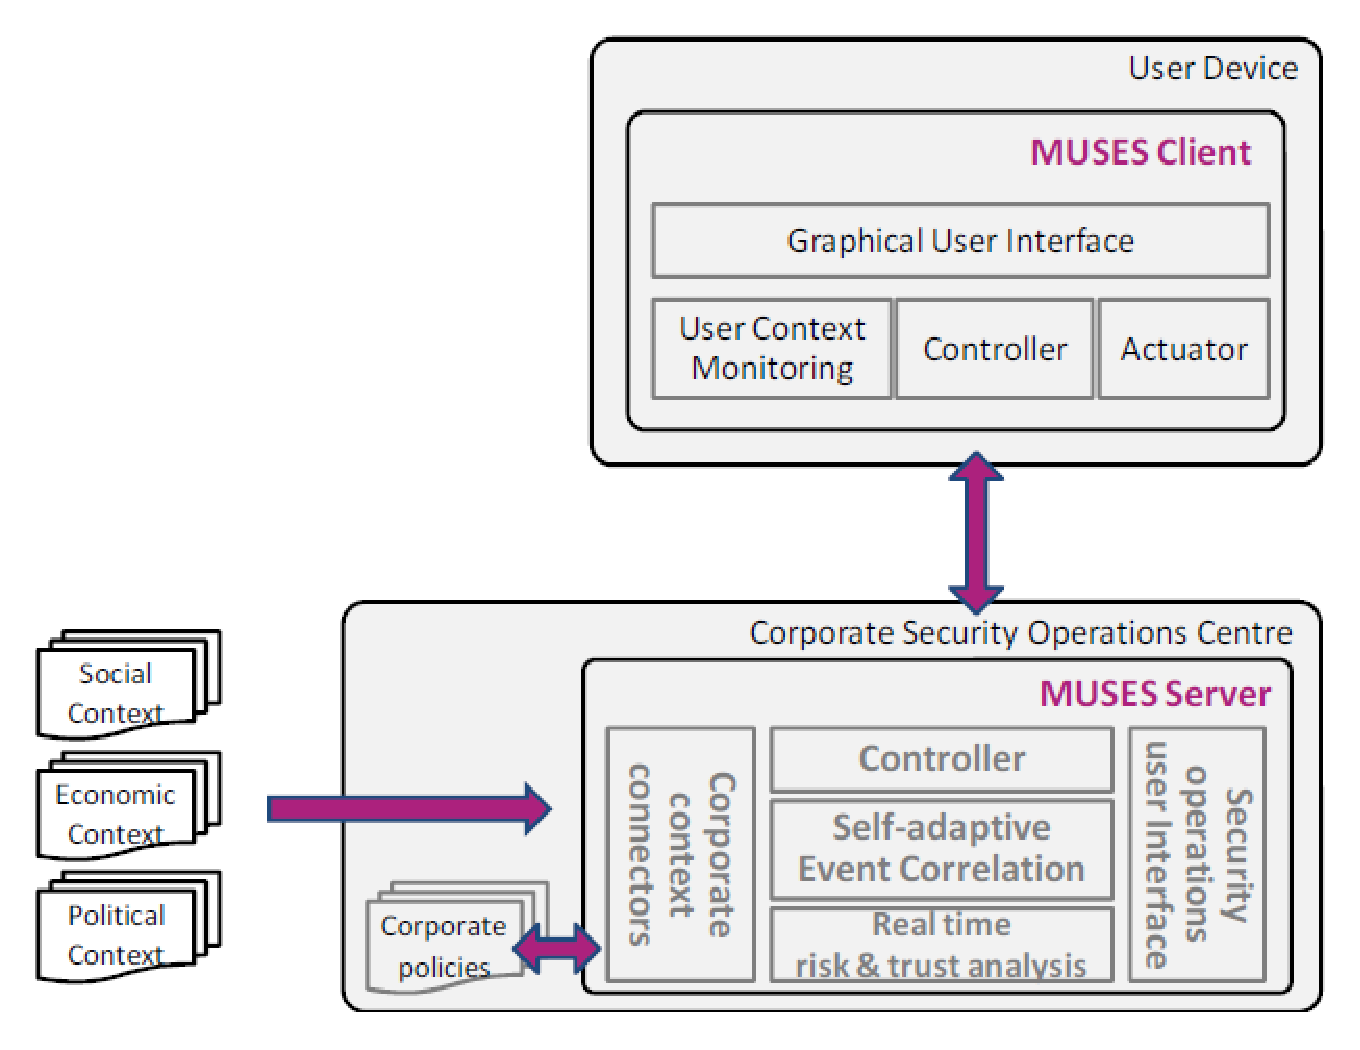
\epsfig{file=architecture.eps, scale=0.38}
\caption{Proposed architecture\label{fig:architecture}}
\end{figure}

One of the main features of the presented system is the self-adaptation (to the user and context) of the set of rules. To this aim, asynchronously to the system working, there will be run a process which will consider the whole amount of historic information regarding user's behaviour and context, and refine it by means of computational intelligence and machine learning techniques. Thus the set of security rules will be adapted to the every user in the system, updating some of the existent rules and creating new ones (always respecting the corporate security policies).
Moreover, some predictive models will be also obtained applying other soft computing techniques, so the user's potentially dangerous behaviour will be anticipated.

%\begin{table}
%\centering
%\caption{Frequency of Special Characters}
%\begin{tabular}{|c|c|l|} \hline
%Non-English or Math&Frequency&Comments\\ \hline
%\O & 1 in 1,000& For Swedish names\\ \hline
%$\pi$ & 1 in 5& Common in math\\ \hline
%\$ & 4 in 5 & Used in business\\ \hline
%$\Psi^2_1$ & 1 in 40,000& Unexplained usage\\
%\hline\end{tabular}
%\end{table}

%\begin{table*}
%\centering
%\caption{Some Typical Commands}
%\begin{tabular}{|c|c|l|} \hline
%Command&A Number&Comments\\ \hline
%\texttt{{\char'134}alignauthor} & 100& Author alignment\\ \hline
%\texttt{{\char'134}numberofauthors}& 200& Author enumeration\\ \hline
%\texttt{{\char'134}table}& 300 & For tables\\ \hline
%\texttt{{\char'134}table*}& 400& For wider tables\\ \hline\end{tabular}
%\end{table*}
% end the environment with {table*}, NOTE not {table}!

%\begin{figure*}
%\centering
%\epsfig{file=flies.eps}
%\caption{A sample black and white graphic (.eps format)
%that needs to span two columns of text.}
%\end{figure*}


%
%%%%%%%%%%%%%%%%%%%%%%%%%%%%%   MUSES Advantages   %%%%%%%%%%%%%%%%%%%%%%%%%%%%%
%
\section{MUSES Advantages}
\label{sec:advantages}

%Inside corporate security, and because of the introduction in the companies of the Bring Your Own Device (BYOD) philosophy, many projects and products have raised to cover this new situation. MUSES is one of these projects, thus the products that have influenced it and which form a solid State of the Art in BYOD security are going to be presented.

There are available some products similar to MUSES, included in the so-called Software-as-a-Service (known SaaS). The most extended are the IBM's \textit{Hosted Mobile Device Security Management} solution, %\cite{IBM_tool} 
Sophos's \textit{Mobile Control} software solution, 
\cite{Sophos_tool}, 
and the \textit{Bring Your Own Device Solution}
\cite{Good_tool} 
of Good Technology. There are other two important products: one exclusive for Samsung devices, the \textit{KNOX} system,
\cite{Samsung_tool}, 
based on separate environments (personal and corporate, for instance), and one exclusive for Blackberry smartphones, the so called \textit{Blackberry Balance}.
\cite{Blackberry_tool}. 

The main differences with MUSES, is that it will be also a free, open-source, platform independent solution. This is an important advantage because all the existent tools take into account only smartphones and tablets, but MUSES covers laptops and company PCs too. Moreover the companies need specific operative system and server (like Windows Server, for instance). Other big plus of the MUSES system is its new feature of self-adaptiveness. MUSES is able to adapt to changes, either regarding corporate security policies, newly discovered vulnerabilities or threats, different environments of use or user profiles. 

In addition, the existing products are mostly policy-based, but MUSES takes its decisions not only considering policies, but also based on the terminals/users context (location, connected networks and so on), to really understand the real danger of a specific action.


%ACKNOWLEDGMENTS are optional
\section{Acknowledgments}
This work has been supported by the MUSES European project (FP7-318508).

%
% The following two commands are all you need in the
% initial runs of your .tex file to
% produce the bibliography for the citations in your paper.
\bibliographystyle{abbrv}
\bibliography{muses_overview}  % sigproc.bib is the name of the Bibliography in this case
% You must have a proper ".bib" file
%  and remember to run:
% latex bibtex latex latex
% to resolve all references
%
% ACM needs 'a single self-contained file'!
%
% That's all folks!
\end{document}
